\documentclass[conference]{IEEEtran}
\IEEEoverridecommandlockouts
\usepackage{cite}
\usepackage{amsmath,amssymb}
\usepackage{graphicx}
\usepackage{booktabs}
\usepackage{xcolor}
\usepackage{array}
\usepackage{tikz}
\usepackage{pgfplots}
\pgfplotsset{compat=1.17}
\usetikzlibrary{positioning,arrows.meta,fit,backgrounds,calc}
\usepackage[hidelinks]{hyperref}

\definecolor{ink}{HTML}{2B2B2B}      \definecolor{inkmuted}{HTML}{6B6A66}
\definecolor{llmfill}{HTML}{E3EEFB}  \definecolor{detfill}{HTML}{FDEBDF}
\definecolor{storefill}{HTML}{F1F0EC}\definecolor{detline}{HTML}{C4501F}
\definecolor{rejline}{HTML}{B3261E}  \definecolor{okline}{HTML}{1B7F4C}
\definecolor{bandA}{HTML}{FAFAF8}    \definecolor{bandB}{HTML}{F4F7FB}
\newcommand{\stg}[1]{\tikz[baseline=-0.6ex]\node[draw=detline,fill=white,circle,inner sep=0.8pt,minimum size=4mm,font=\scriptsize\bfseries]{#1};$\!\to$}
\newcommand{\stgl}[1]{\tikz[baseline=-0.6ex]\node[draw=detline,fill=llmfill,circle,inner sep=0.8pt,minimum size=4mm,font=\scriptsize\bfseries]{#1};}
\newcommand{\sn}[1]{\tikz[baseline=-0.6ex]\node[circle,fill=detline,text=white,inner sep=0.5pt,minimum size=3.2mm,font=\tiny\bfseries]{#1};}

\newcommand{\fw}{\textsc{Trust-RIC}}
\newcommand{\repo}{\url{https://github.com/ahmedchakroun0/Network-Slicing-PoC}}

\newtheorem{proposition}{Proposition}
\newcommand{\G}{\mathcal{G}}
\renewcommand{\IEEEbibitemsep}{0pt plus 0.5pt}

\begin{document}


\title{\fw{}: Trust-Gated Multi-Agent LLM\\ Control for O-RAN Slicing}

\author{
  \IEEEauthorblockN{Ahmed Chakroun $^{1,3}$, Rihab Boussada$^{2,3}$, Le\"\i la Nasraoui$^{1,3}$, Carla Fabiana Chiasserini$^{4}$\\}
  \IEEEauthorblockA{
  $ ^{1}$COSIM Research Lab, Higher School of Communications (SUP'COM), University of Carthage, Tunisia\\
   $ ^{2}$CRISTAL Laboratory, 
$ ^{3}$ National School of Computer Sciences (ENSI) University of Manouba, Tunisia\\
Politecnico di Torino, Turin, Piedmont, Italy\\
emails :
\{ahmedbenmondher.chakroun,rihab.boussada\}@ensi-uma.tn, leila.nasraoui@supcom.tn, carla.chiasserini@polito.it}
}

\maketitle

\begin{abstract}
Large language model (LLM) agents are emerging as controllers for Open Radio Access Networks (O-RAN), but their tool calls may contain hallucinated identifiers, invalid parameters, or unjustified actions that degrade network slices. Existing guardrails primarily constrain dialogue, while agentic RAN frameworks may rely on additional LLM agents to verify proposed actions, leaving network-modifying operations vulnerable to structural and semantic errors. This paper presents \fw{}, a multi-agent architecture for LLM trustworthiness control of RAN slice assurance. \fw{} separates deterministic KPI grounding and trusted-context construction from LLM orchestration and Near-RT/Non-RT RIC action proposal. Every network-modifying tool call passes through a five-stage, fail-closed Trust \& Governance gate that validates the proposed action against code-generated network facts and operational constraints. An LLM-based review provides an additional authorization check at the final stage but cannot override any rejection issued by the deterministic stages. 
%%We run the complete system with a live LLM on slice records derived from ColO-RAN, a dataset collected on a real srsRAN stack (724{,}086 one-second windows, 7 base stations), and score every decision with reproducible rule-based checks. 
We run an end-to-end evaluation comprising 11 records containing violations and 52 tool calls, the gate rejected 56\% of the calls and held every invariant: no rejected call executed, no executed call left its cell and slice, and no executed Physical Resource Block share contradicted the slice policy in force. The LLM orchestrator routed every violation correctly but labelled 8 of 11 violated records ``normal'', which code overrides. Compact prompts and a call budget cut the cost from 117\,k to 86\,k tokens per record, 83\% of the output being hidden reasoning. The evaluation code is available at \repo.
\end{abstract}

\begin{IEEEkeywords}
AI-Native 6G, O-RAN, RAN slicing, agentic AI, large language models, RIC, trustworthy network automation.
\end{IEEEkeywords}

\section{Introduction}
Sixth-generation (6G) networks are envisioned as AI-native systems in which intelligence is embedded into network management, resource allocation, and service orchestration. Large language models (LLMs) are gaining attention as a means of translating operator intents into network configurations and coordinating autonomous control agents \cite{maatouk2025llm,zhou2024llmtelecom,yao2023react}. Recent studies investigate LLM-based orchestration in O-RAN \cite{li2026llmoran}, hierarchical agent architectures \cite{elkael2025agentran,navidan2026multiscale}, and LLM-assisted network management.

O-RAN supports programmable RAN control through the Near-real-time RAN Intelligent Controller (Near-RT RIC), operating over 10\,ms--1\,s timescales, and the Non-real-time RIC (Non-RT RIC), operating over longer timescales \cite{polese2023oran,bonati2021intelligence}. %Network slicing is a key application that requires dynamic resource allocation while maintaining slice-specific service-level agreements (SLAs). Existing work addresses SLA-driven slicing \cite{dai2025oranslicing}, learning-based slicing and scheduling \cite{polese2023coloran}, xApp conflicts \cite{adamczyk2023conflict}, and zero-touch network management \cite{benzaid2020zsm}. However, LLM-driven control introduces risks, including hallucinated parameters, prompt injection, and inconsistent outputs \cite{ji2023hallucination,greshake2023injection}. These issues can result in invalid or unauthorized control actions that compromise network operation and violate SLAs. Existing agentic RAN frameworks explore hierarchical coordination and verification agents \cite{elkael2025agentran,navidan2026multiscale,singh2025assurance}. Meanwhile, programmable guardrails constrain LLM interactions \cite{rebedea2023nemo}, but conversational constraints alone cannot guarantee that control actions are grounded in trusted network state or comply with authorization policies.
Network slicing is a key application that requires dynamic resource allocation while maintaining slice-specific service-level agreements (SLAs). %This induces coordinated control decisions accounting for heterogeneous service requirements, shared radio resources, and operational policies across cells and slices. 
To achieve this, existing work addresses SLA-driven slicing \cite{dai2025oranslicing}, learning-based slicing and scheduling \cite{polese2023coloran}, xApp conflicts \cite{adamczyk2023conflict}, and zero-touch network management \cite{benzaid2020zsm}. However, the emergence of LLM-driven control introduces a different challenge: network actions are increasingly generated through probabilistic reasoning and agent-mediated tool calls rather than exclusively through predefined control logic. Such calls may contain hallucinated parameters, prompt-injected instructions, or inconsistent decisions \cite{ji2023hallucination,greshake2023injection}, potentially resulting in invalid or unauthorized operations that compromise network operation and violate SLAs. Consequently, ensuring that agent-generated actions are grounded in the actual network state and comply with operational policies becomes a fundamental requirement for trustworthy RAN control. Existing agentic RAN frameworks explore hierarchical coordination and verification agents \cite{elkael2025agentran,navidan2026multiscale,singh2025assurance}. Meanwhile, programmable guardrails constrain LLM interactions \cite{rebedea2023nemo}, but conversational constraints alone cannot guarantee that network-modifying actions are grounded in trusted network state or comply with authorization policies.

This paper presents \fw{}, a framework for trustworthy multi-agent LLM control of RAN slice assurance. It embeds deterministic components that construct trusted context and compute SLA-related facts, while LLM agents propose actions that undergo a separate, fail-closed authorization process.
Our contributions are thus as follows:\\
\noindent\textbullet\,\textbf{Architecture:} %(Fig.~\ref{fig:arch}, Sec.~\ref{sec:arch}): 
A multi-agent RAN control framework separating LLM-generated proposals from deterministic authorization, with actions subject to a separate governance gate.

\noindent\textbullet\,\textbf{Trust-gated execution:} A five-stage authorization pipeline with a formal guarantee that LLM review cannot override a rejection by deterministic checks (Sec.~\ref{sec:mono}).
%\noindent\textbullet\, \textbf{Live evaluation with reproducible scoring:} %(Sec.~\ref{sec:eval}).The complete system runs with a live LLM on ColO-RAN records \cite{polese2023coloran}; deterministic checks score SLA detection, interpretation, tool choice, grounding, governance and cost on the stored records.

\noindent\textbullet\,\textbf{Live LLM evaluation with reproducible scoring:} Complete framework evaluation using a live LLM on ColO-RAN records \cite{polese2023coloran}. Each record is assessed using deterministic checks that measure interpretation accuracy, tool selection, context grounding, governance compliance, and token cost.

%, with code and scripts released at \repo.


\begin{figure}[!t]
\centering
\resizebox{0.85\columnwidth}{!}{% Fig. 1 -- target scenario and crucial point (TikZ; editable in Overleaf).
% Requires: tikz libraries positioning, arrows.meta, calc
% and the colours/macros defined in the preamble of main.tex.
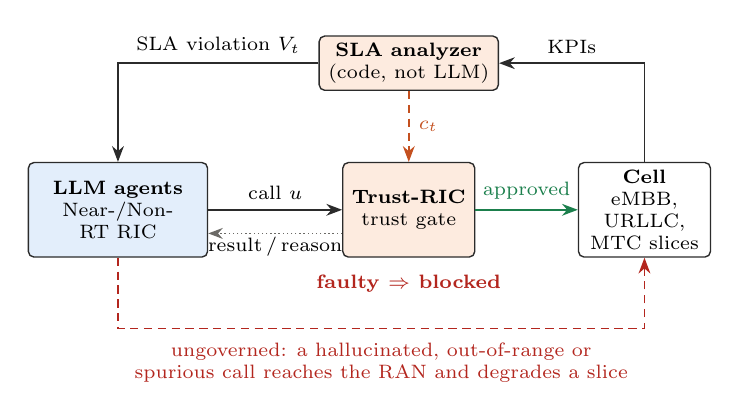
\begin{tikzpicture}[
  font=\scriptsize, >=Stealth,
  box/.style={draw=ink, rounded corners=2pt, align=center, inner sep=2.5pt, line width=0.5pt, fill=white},
  llm/.style={box, fill=llmfill},
  det/.style={box, fill=detfill},
  ctx/.style={->, densely dashed, line width=0.6pt, draw=detline},
]
% ---------- main chain: LLM agents -> gate -> cell
\node[llm, text width=21mm, minimum height=12mm] (ag) at (0,0) {\textbf{LLM agents}\\Near-/Non-RT RIC};
\node[det, text width=15mm, minimum height=12mm, right=17mm of ag] (gt) {\textbf{\fw{}}\\trust gate};
\node[box, text width=15mm, minimum height=12mm, right=13mm of gt] (cell) {\textbf{Cell}\\eMBB, URLLC,\\MTC slices};
% ---------- deterministic SLA analyzer (facts + trusted context)
\node[det, text width=21mm, above=9mm of gt] (sla) {\textbf{SLA analyzer}\\(code, not LLM)};

\draw[->, line width=0.6pt, draw=ink] (ag) -- node[above]{call $u$} (gt);
\draw[->, line width=0.6pt, draw=okline] (gt) -- node[above, text=okline]{approved} (cell);
% KPIs up to the analyzer, facts down to the agents, trusted context to the gate
\draw[->, line width=0.6pt, draw=ink] (cell.north) |- node[pos=0.75, above]{KPIs} (sla.east);
\draw[->, line width=0.6pt, draw=ink] (sla.west) -| node[pos=0.25, above]{SLA violation $V_t$} (ag.north);
\draw[ctx] (sla.south) -- node[right, text=detline]{$c_t$} (gt.north);

% ---------- failure path without a gate
\coordinate (b1) at ([yshift=-9mm]ag.south);
\coordinate (b2) at ([yshift=-9mm]cell.south);
\draw[->, line width=0.6pt, densely dashed, draw=rejline] (ag.south) -- (b1) -- (b2) -- (cell.south);
\node[text=rejline, align=center, below=0.6mm of $(b1)!0.5!(b2)$, font=\scriptsize]
  {ungoverned: a hallucinated, out-of-range or\\spurious call reaches the RAN and degrades a slice};
\node[text=rejline, font=\scriptsize\bfseries, below=1mm of gt] {faulty $\Rightarrow$ blocked};
% ---------- gate returns the outcome to the agent (result if approved, reason if rejected)
\draw[->, line width=0.5pt, densely dotted, draw=inkmuted]
  ([yshift=-3mm]gt.west) -- node[below, font=\tiny, inner sep=1pt]{\scriptsize result\,/\,reason} ([yshift=-3mm]ag.east);
\end{tikzpicture}}
\caption{\fw{} governance workflow for LLM-driven RAN control, enforcing code-based validation and authorization of every control call.}
\label{fig:scenario}
\end{figure}

\begin{figure*}[!t]
\centering
\resizebox{0.85\textwidth}{!}{% Fig. 1 -- system architecture (TikZ; editable in Overleaf).
% Requires: tikz libraries positioning, arrows.meta, fit, backgrounds, calc
% and the colours/macros defined in the preamble of main.tex.
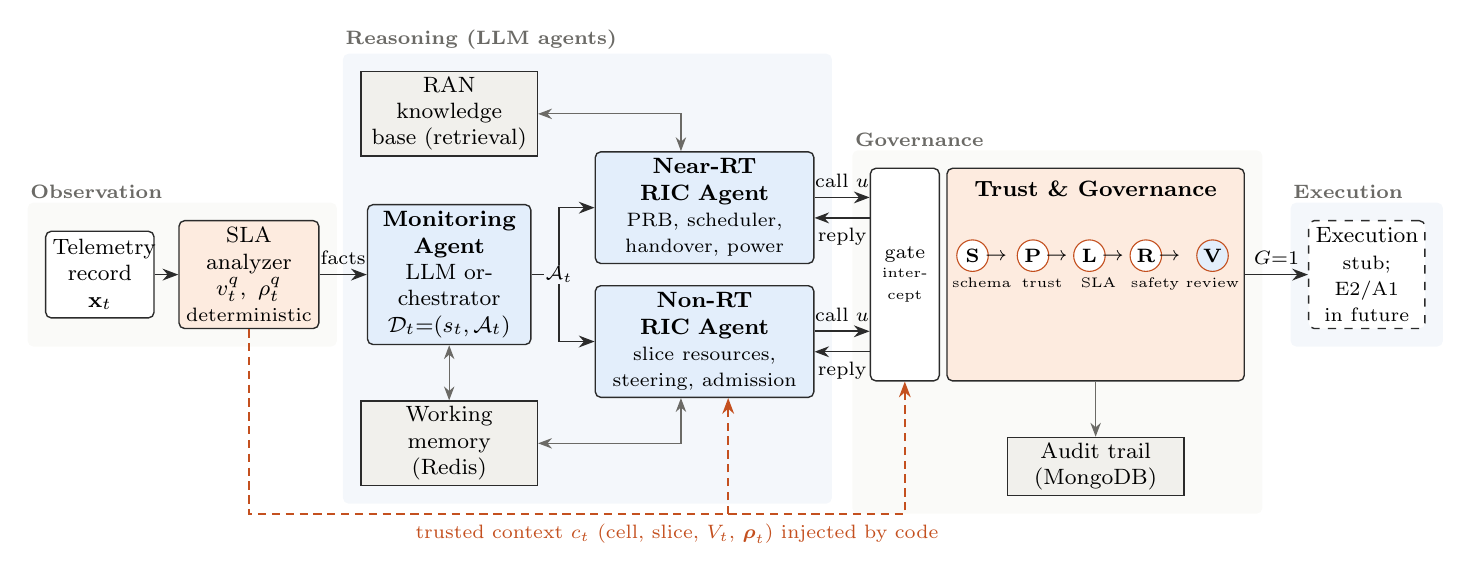
\begin{tikzpicture}[
  font=\footnotesize, >=Stealth,
  box/.style={draw=ink, rounded corners=2pt, align=center, inner sep=2.5pt, line width=0.5pt, fill=white},
  llm/.style={box, fill=llmfill},
  det/.style={box, fill=detfill},
  store/.style={box, fill=storefill, rounded corners=0pt, inner sep=2pt},
  ctx/.style={->, densely dashed, line width=0.6pt, draw=detline},
  flow/.style={->, line width=0.6pt, draw=ink},
  aux/.style={<->, line width=0.45pt, draw=inkmuted},
  lay/.style={font=\scriptsize\bfseries, text=inkmuted, inner sep=1pt},
]
% ---------- observation
\node[box, text width=12mm, minimum height=11mm] (tel) at (0,0) {Telemetry\\record $\mathbf{x}_t$};
\node[det, text width=16mm, minimum height=11mm, right=3mm of tel] (sla) {SLA analyzer\\$v_t^q,\ \rho_t^q$\\{\scriptsize deterministic}};
% ---------- reasoning
\node[llm, text width=19mm, minimum height=11mm, right=6mm of sla] (mon) {\textbf{Monitoring Agent}\\LLM orchestrator\\$\mathcal{D}_t{=}(s_t,\mathcal{A}_t)$};
\node[llm, text width=26mm, anchor=west] (near) at ([xshift=8mm, yshift=8.5mm]mon.east) {\textbf{Near-RT RIC Agent}\\{\scriptsize PRB, scheduler, handover, power}};
\node[llm, text width=26mm, anchor=west] (non) at ([xshift=8mm, yshift=-8.5mm]mon.east) {\textbf{Non-RT RIC Agent}\\{\scriptsize slice resources, steering, admission}};
% ---------- governance
\node[box, text width=7mm, minimum height=27mm, anchor=west, font=\scriptsize] (mw) at ([xshift=7mm]$(near.east)!0.5!(non.east)$) {gate\\[1pt]{\tiny inter-\\cept}};
\node[det, text width=36mm, minimum height=27mm, anchor=west] (gov) at ([xshift=0.8mm]mw.east) {};
\node[anchor=north, font=\footnotesize\bfseries, align=center, yshift=-0.5mm] at (gov.north) {Trust \& Governance};
\node[anchor=center, font=\scriptsize] at ([yshift=1mm]gov.center)
 {\setlength{\tabcolsep}{1pt}\begin{tabular}{@{}ccccc@{}}
   \stg{S}&\stg{P}&\stg{L}&\stg{R}&\stgl{V}\\
   {\tiny schema}&{\tiny trust}&{\tiny SLA}&{\tiny safety}&{\tiny review}
  \end{tabular}};

% ---------- execution
\node[box, dashed, text width=13mm, minimum height=11mm, right=8mm of gov] (exe) {Execution\\{\scriptsize stub; E2/A1 in future}};
% ---------- stores
\node[store, text width=21mm, anchor=north] (wm) at ([yshift=-7mm]mon.south) {Working memory\\(Redis)};
\node[store, text width=21mm, anchor=north] (db) at ([yshift=-7mm]gov.south) {Audit trail\\(MongoDB)};
\node[store, text width=21mm, anchor=south] (kb) at ([yshift=6mm]mon.north) {RAN knowledge\\base (retrieval)};

% ---------- main flows
\draw[flow] (tel) -- (sla);
\draw[flow] (sla) -- node[above, font=\scriptsize]{facts} (mon);
\draw[flow] (mon.east) -- ++(3.5mm,0) |- (near.west);
\draw[flow] (mon.east) -- ++(3.5mm,0) |- (non.west);
\node[font=\scriptsize, fill=bandB, inner sep=0.5pt] at ([xshift=3.5mm]mon.east) {$\mathcal{A}_t$};
\draw[flow] ([yshift=1.3mm]near.east) -- node[above, font=\scriptsize]{call $u$} ([yshift=1.3mm]near.east -| mw.west);
\draw[flow] ([yshift=1.3mm]non.east) -- node[above, font=\scriptsize]{call $u$} ([yshift=1.3mm]non.east -| mw.west);
\draw[->, line width=0.5pt, draw=ink] ([yshift=-1.3mm]near.east -| mw.west) -- node[below, font=\scriptsize]{reply} ([yshift=-1.3mm]near.east);
\draw[->, line width=0.5pt, draw=ink] ([yshift=-1.3mm]non.east -| mw.west) -- node[below, font=\scriptsize]{reply} ([yshift=-1.3mm]non.east);
\draw[flow] (gov.east) -- node[above, font=\scriptsize]{$G{=}1$} (exe.west);
% ---------- trusted context (deterministic, overrides LLM-written context)
\coordinate (cy) at ([yshift=-3.5mm]wm.south);
\draw[ctx] (sla.south) |- (cy) -| node[pos=0.25, below, font=\scriptsize, text=detline]{trusted context $c_t$ (cell, slice, $V_t$, $\boldsymbol\rho_t$) injected by code} (mw.south);
\draw[ctx] ([xshift=3mm]non.south |- cy) -- ([xshift=3mm]non.south);
% ---------- memory, audit, knowledge
\draw[aux] (mon.south) -- (wm.north);
\draw[aux] (wm.east) -| ([xshift=-3mm]non.south);
\draw[->, line width=0.45pt, draw=inkmuted] (gov.south) -- (db.north);
\draw[aux] (kb.east) -| ([xshift=-3mm]near.north);

% ---------- layer bands
\begin{scope}[on background layer]
 \node[fit=(tel)(sla), inner sep=2.2mm, fill=bandA, rounded corners=2pt] (L1) {};
 \node[fit=(mon)(near)(non)(kb)(wm), inner sep=2.2mm, fill=bandB, rounded corners=2pt] (L2) {};
 \node[fit=(mw)(gov)(db), inner sep=2.2mm, fill=bandA, rounded corners=2pt] (L3) {};
 \node[fit=(exe), inner sep=2.2mm, fill=bandB, rounded corners=2pt] (L4) {};
\end{scope}
\node[lay, anchor=south west] at (L1.north west) {Observation};
\node[lay, anchor=south west] at (L2.north west) {Reasoning (LLM agents)};
\node[lay, anchor=south west] at (L3.north west) {Governance};
\node[lay, anchor=south west] at (L4.north west) {Execution};
\end{tikzpicture}
}
\caption{The \fw{} architecture. Deterministic components produce facts and the trusted context, LLM agents orchestrate and propose actions, and every protected tool call is authorized before execution. Each record runs once through this workflow.}
\label{fig:arch}
\end{figure*}



The remaining of this paper is organized as follows. Section II describes the system model and defines the problem statement. The proposed \fw{} framework is introduced in Section III, then evaluated in Section IV. Finally, the paper concludes in Section V. 


% =====================================================================
\section{System Model and Problem Statement}\label{sec:model}
\noindent Consider an AI-native O-RAN architecture where LLM-based agents monitor SLA compliance and propose RAN control actions through Near-RT and Non-RT RICs as shown in Fig.~\ref{fig:scenario}. We here define the SLA model, violation detection mechanism, available control actions, and requirements for trustworthy action authorization.

% \noindent \textbf{SLA facts.} At step $t$, a record $\mathbf{x}_t$ describes one slice of one cell over a one-second window. Its SLA KPIs are $q\!\in\!\mathcal{Q}\!=\!\{\text{thr},\text{del}\}$: the downlink throughput per user equipment (UE), $m_t^{\text{thr}}$, and the queueing delay $m_t^{\text{del}}$, i.e., the downlink backlog divided by the delivered rate. The budgets $b^q$ depend on the slice (Sec.~\ref{sec:eval}). The SLA analyzer computes

\noindent \textbf{SLA facts.} At step $t$, a record $\mathbf{x}_t$ describes one slice of one cell over a one-second window.Its SLA KPIs are $q\!\in\!\mathcal{Q}\!=\!\{\text{thr},\text{del}\}$, where thr denotes the downlink throughput per user equipment (UE), $m_t^{\text{thr}}$ (Mbps), and del the queueing delay, $m_t^{\text{del}}$ (ms), i.e., the downlink backlog divided by the delivered rate. The budgets $b^q$ depend on the slice (Sec.~\ref{sec:eval}): a minimum for thr and a maximum for del. The SLA analyzer computes

\begin{equation}
v_t^q=\begin{cases}\mathbb{1}[m_t^q<b^q] & q=\text{thr}\\ \mathbb{1}[m_t^q>b^q] & q=\text{del}\\ \bot & m_t^q\text{ missing,}\end{cases}
\end{equation}
the violation set $V_t=\{q: v_t^q=1\}$, and the persistence $\rho_t^q=(\rho_{t-1}^q+1)\,v_t^q$, counted per (cell, slice) stream. Unavailable KPIs ($\bot$) are treated as neither healthy nor violated.





\noindent \textbf{RIC control.} A RIC agent $a$ owns tools $\mathcal{T}_a$. Near-RT tools set a slice's Physical Resource Block (PRB) share, the MAC scheduler, the QoS parameters (priority, packet delay budget, guaranteed bit rate), the link adaptation (modulation and coding scheme (MCS) offset, target Block Error rate (BLER)), the handover margin and the power offset. The Non-RT tool sets the slice resource policy: a guaranteed and a capped PRB share. A tool call is $u=(\tau,\theta,r)$, with tool $\tau$, parameters $\theta$ and reasoning $r$ (rationale, expected effect, confidence, evidence).

\noindent \textbf{Problem.} The calls $u$ are produced by an LLM and may be (i) structurally invalid (hallucinated identifier, extra or missing argument), (ii) out of range or inverted, (iii) unjustified (no violation, wrong slice or wrong role), (iv) inconsistent with the controls already in force, or (v) well-formed but semantically wrong. We seek a decision $\G\in\{0,1\}$ on each call, taken before execution, that blocks (i)--(iv) without rejecting valid calls, cannot be widened by the LLM, and costs far less than the Near-RT budget. Class (v) is beyond deterministic checks and is what the LLM review targets.

% =====================================================================
\section{The \fw{} Framework}\label{sec:arch}

\subsection{Overview and agents}\label{sec:agents}
\noindent \fw{} (\emph{Trust-gated RIC agents}) is a multi-agent architecture that keeps O-RAN network slices within their SLAs. Its key idea is a separation of duties: LLM agents interpret SLA violations and propose control actions, while deterministic code computes the facts these agents rely on and authorizes every action before it reaches the RAN.

\noindent Fig.~\ref{fig:arch} shows the architecture as four layers, traversed from left to right by each telemetry record. In the \emph{observation} layer, a deterministic SLA analyzer compares the record with the budgets of its slice and computes which KPIs are violated and for how many consecutive records. In the \emph{reasoning} layer, three LLM agents decide how to react. In the \emph{governance} layer, a trust gate intercepts every action proposed by these agents and authorizes or rejects it. In the \emph{execution} layer, approved actions are applied to the RAN.

\noindent The agents, summarized in Table~\ref{tab:agents}, each have a single responsibility:
\begin{itemize}
\item \textbf{Monitoring agent}, the entry point of the reasoning layer. For each violated record, it describes the situation, rates its severity and decides which RIC agents to invoke, giving each one an objective. It has no tool: it can only delegate, never act.
\item \textbf{Near-RT RIC agent}, which applies fast, local fixes on the violated slice of one cell through six action tools: the PRB share, the scheduler, the QoS parameters, the link adaptation, the handover margin and the power offset.
\item \textbf{Non-RT RIC agent}, which sets the longer-term slice resource policy (guaranteed and capped PRB share). It is invoked only when a violation has persisted for at least three records, and runs after the Near-RT agent so that the policy and the latest allocation agree.
\item \textbf{Trust \& Governance agent}, which is not a peer of the others but the authority between the RIC agents and the RAN. Every action call of a RIC agent is intercepted and checked, first by deterministic stages and then by an LLM review; the decision and its reason are returned to the calling agent and recorded.
\end{itemize}
The agents thus form a chain: the Monitoring agent delegates, the RIC agents propose, and the gate authorizes. No agent can skip the next one, and none executes an action by itself. Three shared resources support them: a RAN knowledge base on O-RAN, slicing KPIs and control actions, searched by both RIC agents; a working memory (Redis) holding the recent records and actions of each cell and slice, read by the Monitoring and RIC agents but not by the gate; and an audit store (MongoDB) that keeps every decision with its reason, per record.

\begin{table}[!t]
\centering
\caption{The agents of \fw{}}
\label{tab:agents}
\footnotesize
\setlength{\tabcolsep}{2pt}
\begin{tabular}{@{}>{\raggedright\arraybackslash}p{18mm}>{\raggedright\arraybackslash}p{28mm}>{\raggedright\arraybackslash}p{21mm}>{\raggedright\arraybackslash}p{16mm}@{}}
\toprule
Agent & Role & Reads & Produces \\
\midrule
Monitoring (LLM) & interpret the violation, select the RIC agents, set their objectives & record, SLA facts, working memory & decision $\mathcal{D}_t$ (no tool) \\
Near-RT RIC (LLM) & fast, local mitigation on one cell and slice & objective, $c_t$, working memory, knowledge & calls to 6 action tools \\
Non-RT RIC (LLM) & slice policy for persistent violations ($\rho\ge3$) & same, after the Near-RT agent & calls to the slice resource policy \\
Trust \& Governance (code + LLM review) & authorize each action call & proposal $p$, trusted context $c_t$ & $\G\in\{0,1\}$, stage, reason \\
\bottomrule
\end{tabular}
\end{table}

\subsection{Workflow}
\noindent Each record runs once through the workflow of Fig.~\ref{fig:wf}, implemented as a LangGraph state graph whose state holds the record, its SLA analysis, the Monitoring decision and the agents' results. The workflow has six steps; steps 2--6 appear from top to bottom in Fig.~\ref{fig:wf}, which follows a single tool call:
\begin{itemize}
\item[\sn{1}] \textbf{Ground.} Code turns the record into SLA facts $(v_t^q,V_t,\rho_t^q)$ and builds the trusted context $c_t$ (Sec.~\ref{sec:ctx}). A record without violation ($V_t=\emptyset$) ends here, without any LLM call.
\item[\sn{2}] \textbf{Route.} The Monitoring agent reads the record, the SLA facts and the working memory, and returns its decision $\mathcal{D}_t$: a situation, a severity, the RIC agents to invoke and an objective for each. Code then corrects the decision where it contradicts the facts: it sets the computed severity, never lets a violated record be called ``normal'', drops the Non-RT agent unless $\max_{q\in V_t}\rho_t^q\ge3$, and invokes the Near-RT agent if no agent is left.
\item[\sn{3}] \textbf{Propose.} The selected RIC agents run in a fixed order, Near-RT first, so that the Non-RT agent sees the actions just taken. Each agent reads the working memory of its cell and slice, may search the knowledge base, and emits tool calls $u$ with its reasoning.
\item[\sn{4}] \textbf{Authorize.} Each action call is intercepted before it runs, turned into a proposal $p$ carrying $c_t$, and checked by the gate (Sec.~\ref{sec:mono}), which returns $\G\in\{0,1\}$.
\item[\sn{5}] \textbf{Execute or reject.} If $\G{=}1$, the tool runs and its result returns to the agent. If $\G{=}0$, the reason of the rejection returns to the agent, which may revise its call or stop.
\item[\sn{6}] \textbf{Audit.} Every call is recorded as it happens, with the agent's rationale, expected effect and evidence, the gate's decision and reason, and the outcome. The working memory receives structured facts only, never LLM text.
\end{itemize}

\begin{figure}[!t]
\centering
\resizebox{0.95\columnwidth}{!}{% Fig. 2 -- governed tool-call workflow (sequence view; TikZ)
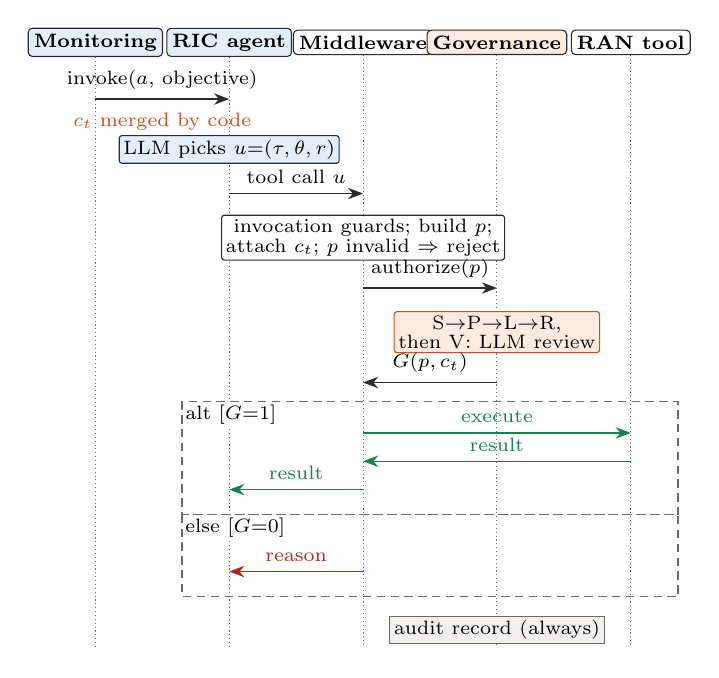
\begin{tikzpicture}[
  font=\scriptsize, >=Stealth, yscale=0.8,
  hd/.style={draw=ink, rounded corners=1.5pt, fill=#1, inner sep=2pt, minimum width=11mm, align=center, font=\scriptsize\bfseries},
  life/.style={draw=inkmuted, densely dotted, line width=0.4pt},
  msg/.style={->, line width=0.55pt, draw=ink},
  rej/.style={->, line width=0.55pt, draw=rejline},
  ok/.style={->, line width=0.55pt, draw=okline},
  frame/.style={draw=inkmuted, densely dashed, line width=0.4pt},
  tag/.style={font=\scriptsize, anchor=north west, fill=white, inner sep=1pt},
  act/.style={draw=detline, fill=detfill, inner sep=1.5pt, align=center, rounded corners=1pt, font=\scriptsize},
]
\def\H{-94mm}
\foreach \x/\n/\t/\c in {0/M/Monitoring/llmfill, 17/A/RIC agent/llmfill, 34/W/Middleware/white, 51/G/Governance/detfill, 68/T/RAN tool/white}{
  \node[hd=\c] (\n) at (\x mm,0) {\t};
  \draw[life] (\n.south) -- ++(0,\H);
}
% 1
\draw[msg] (0,-9mm) -- node[above]{invoke$(a$, objective$)$} (17mm,-9mm);
\node[font=\scriptsize, text=detline, anchor=north] at (8.5mm,-9.6mm) {$c_t$ merged by code};
% 2
\node[act, fill=llmfill, draw=ink] at (17mm,-17mm) {LLM picks $u{=}(\tau,\theta,r)$};
% 3
\draw[msg] (17mm,-24mm) -- node[above]{tool call $u$} (34mm,-24mm);
\node[act, fill=white, draw=ink] at (34mm,-31mm) {invocation guards; build $p$;\\[-1pt]attach $c_t$; $p$ invalid $\Rightarrow$ reject};
% 4
\draw[msg] (34mm,-39mm) -- node[above]{authorize$(p)$} (51mm,-39mm);
\node[act] at (51mm,-46mm) {S$\to$P$\to$L$\to$R,\\[-1pt]then V: LLM review};
\draw[msg] (51mm,-54mm) -- node[above]{$G(p,c_t)$} (34mm,-54mm);
% 5 alt: approved
\draw[frame] (11mm,-57mm) rectangle (74mm,-75mm);
\node[tag] at (11mm,-57mm) {alt\ [$G{=}1$]};
\draw[ok] (34mm,-62mm) -- node[above, text=okline]{execute} (68mm,-62mm);
\draw[ok] (68mm,-66.5mm) -- node[above, text=okline]{result} (34mm,-66.5mm);
\draw[ok] (34mm,-71mm) -- node[above, text=okline]{result} (17mm,-71mm);
% 6 else: rejected
\draw[frame] (11mm,-75mm) rectangle (74mm,-88mm);
\node[tag] at (11mm,-75mm) {else\ [$G{=}0$]};
\draw[rej] (34mm,-84mm) -- node[above, text=rejline]{reason} (17mm,-84mm);

% audit on the governance lifeline
\node[draw=inkmuted, fill=storefill, inner sep=1.5pt, font=\scriptsize, anchor=north] at (51mm,-91mm) {audit record (always)};
\end{tikzpicture}}
\caption{Workflow of one governed tool call (steps 2--6). The call carries the trusted context supplied by code; the gate approves or rejects it, and every outcome is audited.}
\label{fig:wf}
\end{figure}

\subsection{Trusted context}\label{sec:ctx}
\noindent An LLM agent writes the arguments of its own calls, so it may name a wrong slice or claim a violation that does not exist. To prevent this, code computes the \emph{trusted context} of each record in step~1, before any LLM runs:
\begin{equation}
c_t=(\text{cell},\,\text{slice},\,V_t,\,\boldsymbol{\rho}_t,\,\mathbf{s}_t,\,\kappa_t).
\end{equation}
It contains the cell and slice of the record, the violated KPIs $V_t$ and how long they have lasted ($\boldsymbol{\rho}_t$), the current state of the slice $\mathbf{s}_t$ (e.g., its PRB share and utilization), and the controls in force $\kappa_t$ (the last executed PRB share and slice policy, refreshed before each RIC agent runs). The RIC agents read $c_t$ to know the situation and the scope they act on, and the gate checks every action against it; no LLM can modify it. For example, an action on the URLLC slice is rejected when only eMBB is violated, and a slice policy is rejected if it excludes the PRB share just executed. The working memory complements $c_t$ with the recent history of the cell and slice, but it only informs the agents and is never used by the gate.

\subsection{Authorization}\label{sec:mono}
\noindent Every action call goes through two levels of checks before it can run. First, \emph{invocation guards} reject a call that exceeds the call budget of the invocation, that changes a resource (PRB share, scheduler, QoS, \dots) already changed in the same invocation, or that resubmits a call with the same parameters after the LLM review rejected it, since rewording a rationale does not change the action. Second, the gate evaluates the proposal $p$ against $c_t$:
\begin{equation}
\G(p,c_t)=g_S\,g_P\,g_L\,g_R\cdot g_V \in\{0,1\},
\end{equation}
stage by stage, stopping at the first rejection:
\begin{itemize}
\item $g_S$ (\emph{schema}): the call has exactly the arguments of its tool, and a non-empty rationale and expected effect;
\item $g_P$ (\emph{policy and trust}): the tool belongs to the calling agent ($\tau\in\mathcal{T}_a$), and its cell and slice are those of $c_t$;
\item $g_L$ (\emph{SLA justification}): the record is violated ($V_t\neq\emptyset$), and for a Non-RT policy the violation has persisted ($\max_{q\in V_t}\rho_t^q\ge3$);
\item $g_R$ (\emph{resource safety}): each parameter lies within a safe operating range set by the operator; in our implementation, PRB share $\in[5,90]$\%, scheduler $\in$ \{round robin, waterfilling, proportional fair\}, priority $\in[1,10]$, packet delay budget $\in[5,300]$\,ms, guaranteed bit rate $\in[0,10]$\,Mbps, MCS offset $\in[-5,5]$, target BLER $\in[0.001,0.2]$, handover margin $\in[0,10]$\,dB, power offset $\in[-6,6]$\,dB, policy minimum $\in[5,80]$\% and maximum $\in[20,100]$\% with min$\,\le\,$max, and a tool without such a range is rejected; moreover, a PRB share must lie within the policy in force, and a policy must contain the PRB share in force ($\kappa_t$);
\item $g_V$ (\emph{LLM review}): an LLM judges whether the agent's reasoning is sound, aligned with its objective and appropriate for its role.
\end{itemize}
\noindent The tool runs only if the guards pass and $\G=1$. The LLM review $g_V$ runs only after all the code checks have passed: it can reject a call that the code accepted, but never approve a call that the code rejected, and if it fails (error, timeout or invalid answer), the call is rejected. Since the code checks rely only on $c_t$ and fixed rules, which no LLM can modify, a hallucinated or injected instruction may change what an agent proposes or what $g_V$ answers, but cannot get an action executed outside what the code allows.


% =====================================================================
\section{Performance Evaluation}\label{sec:eval}
\noindent This section evaluates whether \fw{} keeps LLM-driven slice control both effective and safe when the complete system runs with a live LLM on real RAN traces. Sec.~\ref{sec:setup} describes the data, the implementation and the runs, Sec.~\ref{sec:metrics} defines what we measure, and Sec.~\ref{sec:results} presents the results, following the path of a record through the system.

\subsection{Experimental setup}\label{sec:setup}
\noindent \textbf{Dataset.} We use the ColO-RAN dataset \cite{polese2023coloran}, collected on the Colosseum emulator with an srsRAN-based stack in an urban scenario: 7 base stations (BSs) with 10\,MHz (50 PRBs) and three slices each (eMBB at 4\,Mbps CBR per UE, MTC at 30 Poisson packets/s, URLLC at 10 Poisson packets/s), with two static UEs per slice. Each run uses one of three schedulers (round robin, waterfilling, proportional fair) and one of 28 splits of the 17 resource block groups among the slices. We aggregate the 250\,ms per-UE reports into one-second slice records, i.e., the records $\mathbf{x}_t$ of Sec.~\ref{sec:model}, which yields 724{,}086 records (241{,}362 per slice). Each record carries the slice's PRB allocation and utilization, the PRBs left unused by the other slices, the scheduler, the throughput per UE, the queueing delay, CQI, MCS and uplink SINR.

\noindent \textbf{SLA budgets.} To decide which of these records violate their SLA, we derive the budgets from the traffic classes: at least 90\% of the offered load per UE for eMBB (3.6\,Mbps) and 50\% for MTC and URLLC (0.015 and 0.005\,Mbps), and a queueing delay of at most 100\,ms (eMBB, MTC) or 10\,ms (URLLC). With these budgets, 31.2\% of the records are violated: 91.2\% of eMBB, 2.1\% of URLLC and 0.4\% of MTC records. Of the violated records, 92.8\% use at least 90\% of their PRBs and 97.4\% have lasted at least three consecutive records. The agents therefore mostly face persistent eMBB violations caused by a lack of PRBs.

\noindent \textbf{Implementation and model.} We implemented \fw{} in Python~3.12. Each record is processed by a LangGraph workflow, and each agent is a LangChain tool-calling agent whose action tools are intercepted by the gate as a middleware. Exchanged objects are validated with Pydantic, the working memory is kept in Redis, and every decision is stored in MongoDB. All LLM roles (Monitoring, both RIC agents and $g_V$) use NVIDIA Nemotron~3.5 Lightning, a mixture-of-experts model with 30B parameters (3B active), at temperature 0. An approved tool returns a confirmation and the next record is read from the dataset, so the evaluation is open-loop: it measures the decisions of the agents and of the gate.

\noindent \textbf{Runs.} All runs replay the eMBB slice of BS bs2 (round robin, split \texttt{tr2}), which violates both KPIs. We compare two configurations of the same system. In \textbf{R1} (three runs), each RIC agent may make up to 20 action calls per invocation. \textbf{R2} (one run) is an optimized configuration: two action calls per invocation, a more compact working memory and prompt, and a single model call to obtain an action. Two earlier runs, \textbf{R0}, are used only to explain two checks added to the gate.

\subsection{Evaluation metrics}\label{sec:metrics}
\noindent We evaluate the system at three levels. All metrics are computed from the stored decisions by deterministic rules, so they are reproducible and need no LLM judge.

\noindent \textbf{Agents.} Do the agents understand the situation and act sensibly?
\begin{itemize}
\item \emph{Interpretation}: the Monitoring agent's own decision, before code corrects it, is compared with the computed severity, with the routing rule (Near-RT on every violation, Non-RT from $\rho\ge3$), and with the violated KPIs each objective must name.
\item \emph{Tool choice}: the bottleneck of the record is diagnosed (PRB-limited if the PRB utilization is at least 0.9, radio-limited if CQI $<7$), and each call is classified as matching it, neutral (scheduler, QoS) or off-target; a PRB change must also raise the share and fit within the available PRBs.
\item \emph{Grounding}: every number quoted in a rationale must match a value of the agent's context, up to rounding or a simple derivation, and every cited evidence source must be supported by the context or the retrieved knowledge.
\end{itemize}
\noindent \textbf{Gate.} Does the gate stop unsafe actions without blocking the system? We count the calls approved and rejected per stage, check three safety properties (no rejected call is executed, no executed call acts outside its cell and slice, no executed PRB share contradicts the slice policy in force), and measure the decision latency with and without the LLM review.

\noindent \textbf{Cost.} What does LLM control cost? We report the model calls, the input, output and reasoning tokens, and the agent time per violated record.

\begin{table}[!t]
\centering
\caption{Live LLM agents behind the gate (Nemotron~3.5 Lightning; R1: no call cap, R2: two calls, compact prompts)}\label{tab:live}
\footnotesize
\setlength{\tabcolsep}{3pt}
\begin{tabular}{@{}lrr@{}}
\toprule
Metric & R1 & R2 \\
\midrule
Records with a violation & 7 & 4 \\
Violations flagged by the Monitoring LLM (\%) & 100 (7/7) & 100 (4/4) \\
Situation not called normal (\%) & 29 (2/7) & 25 (1/4) \\
Severity agrees with code (\%) & 86 (6/7) & 75 (3/4) \\
Routing agrees with the rule (\%) & 100 (7/7) & 100 (4/4) \\
Protected tool calls per record & 4.6 & 5.0 \\
Tool consistent with the diagnosis (\%) & 55 (11/20) & 83 (10/12) \\
PRB change in the right direction (\%) & 100 (11/11) & 100 (10/10) \\
Quoted numbers traceable (\%) & 98 (483/492) & 99 (256/259) \\
Evidence sources supported (\%) & 96 (94/98) & 85 (29/34) \\
Calls approved (\%) & 53 (17/32) & 30 (6/20) \\
Calls rejected by code (\%) & 31 (10/32) & 55 (11/20) \\
Calls rejected by the LLM review (\%) & 16 (5/32) & 15 (3/20) \\
Review rejection overturned by rewording & 0 & 0 \\
Gate invariant violations & 0 & 0 \\
PRB share outside the slice policy & 0 & 0 \\
Model calls per record & 12.6 & 11.0 \\
Tokens per record, input (k) & 79.2 & 63.6 \\
Tokens per record, output (k) & 37.9 & 22.9 \\
\quad of which reasoning (k) & -- & 19.0 \\
Tokens per record, total (k) & 117.2 & 86.5 \\
RIC phase per record (s) & 501 & 273 \\
\bottomrule
\end{tabular}
\end{table}


\begin{figure}[!t]
\centering
% Generated by scripts/paper_figures.py from tables/live.json -- do not edit.
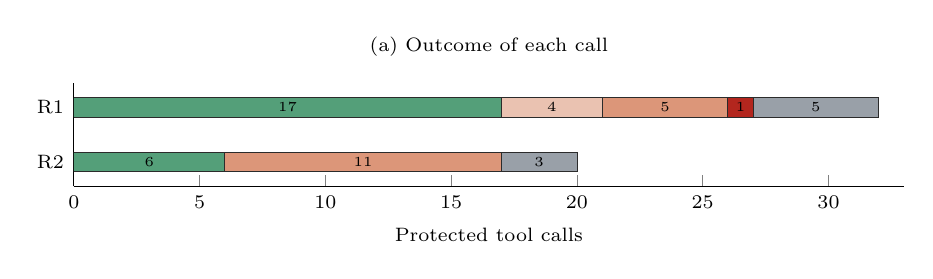
\begin{tikzpicture}
\begin{axis}[xbar stacked, bar width=7pt, axis x line*=bottom, axis y line*=left, tick label style={font=\scriptsize}, label style={font=\scriptsize}, legend style={font=\tiny, draw=none, fill=none, legend columns=-1, /tikz/every even column/.append style={column sep=3pt}}, legend image code/.code={\draw[#1] (0,-0.08) rectangle (0.18,0.1);}, nodes near coords={\pgfmathfloatifflags{\pgfplotspointmeta}{0}{}{\pgfmathprintnumber{\pgfplotspointmeta}}}, point meta=explicit, every node near coord/.append style={font=\tiny}, nodes near coords align={center}, width=\columnwidth, height=2.9cm,
  xmin=0, xmax=33, xlabel={Protected tool calls},
  symbolic y coords={R2,R1}, ytick=data, enlarge y limits=0.45,
  legend to name=legOutcome,
  title={\scriptsize (a) Outcome of each call}]
\addplot[fill=okline!75, draw=ink, line width=0.3pt] coordinates {(17,R1) [17] (6,R2) [6]};
\addlegendentry{Approved}
\addplot[fill=detline!35, draw=ink, line width=0.3pt] coordinates {(4,R1) [4] (0,R2) [0]};
\addlegendentry{Malformed ($g_S$)}
\addplot[fill=detline!60, draw=ink, line width=0.3pt] coordinates {(5,R1) [5] (11,R2) [11]};
\addlegendentry{Guards}
\addplot[fill=rejline, draw=ink, line width=0.3pt] coordinates {(1,R1) [1] (0,R2) [0]};
\addlegendentry{Unsafe ($g_R$)}
\addplot[fill=llmfill!60!ink, draw=ink, line width=0.3pt] coordinates {(5,R1) [5] (3,R2) [3]};
\addlegendentry{LLM review ($g_V$)}
\end{axis}
\end{tikzpicture}\\[-1mm]
\ref{legOutcome}\\[1mm]
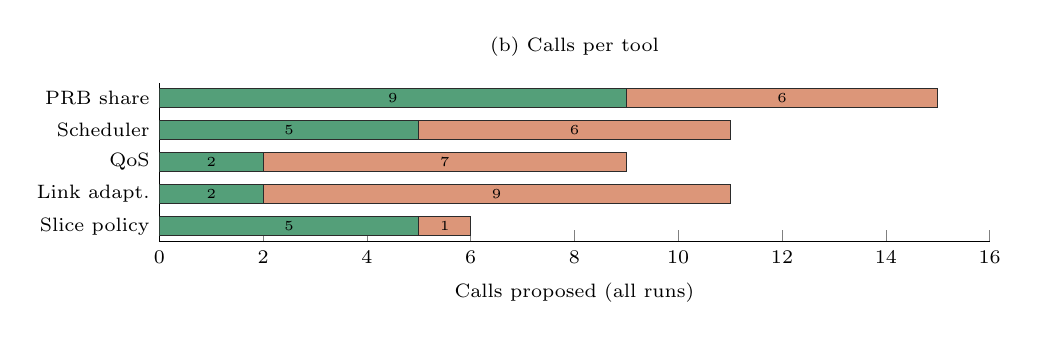
\begin{tikzpicture}
\begin{axis}[xbar stacked, bar width=7pt, axis x line*=bottom, axis y line*=left, tick label style={font=\scriptsize}, label style={font=\scriptsize}, legend style={font=\tiny, draw=none, fill=none, legend columns=-1, /tikz/every even column/.append style={column sep=3pt}}, legend image code/.code={\draw[#1] (0,-0.08) rectangle (0.18,0.1);}, nodes near coords={\pgfmathfloatifflags{\pgfplotspointmeta}{0}{}{\pgfmathprintnumber{\pgfplotspointmeta}}}, point meta=explicit, every node near coord/.append style={font=\tiny}, nodes near coords align={center}, width=\columnwidth, height=3.6cm,
  xmin=0, xmax=16, xlabel={Calls proposed (all runs)},
  symbolic y coords={Slice policy,Link adapt.,QoS,Scheduler,PRB share}, ytick=data, enlarge y limits=0.12,
  legend to name=legTool,
  title={\scriptsize (b) Calls per tool}]
\addplot[fill=okline!75, draw=ink, line width=0.3pt] coordinates {(9,PRB share) [9] (5,Scheduler) [5] (2,QoS) [2] (2,Link adapt.) [2] (5,Slice policy) [5]};
\addlegendentry{Approved}
\addplot[fill=detline!60, draw=ink, line width=0.3pt] coordinates {(6,PRB share) [6] (6,Scheduler) [6] (7,QoS) [7] (9,Link adapt.) [9] (1,Slice policy) [1]};
\addlegendentry{Rejected}
\end{axis}
\end{tikzpicture}\\[-1mm]
\ref{legTool}

\caption{Gate decisions on the 52 live tool calls. (a) Outcome per run: approved, or the stage that rejected the call. (b) Calls per tool over all runs.}
\label{fig:live}
\end{figure}

\subsection{Results}\label{sec:results}
\noindent Table~\ref{tab:live} summarizes the results of both configurations. We follow the path of a record: the agents' decisions, the gate, and finally latency and cost.

\noindent \textbf{Interpretation.} We first check that the Monitoring agent understands the violations it receives. It flagged every violation, routed it as the rule requires in 11/11 records, and named the violated KPIs with correct values in every objective. However, it labelled 8 of the 11 violated records ``normal'' and misjudged 2 severities; code corrected both before any action, which shows why the facts must remain with code.

\noindent \textbf{Tool choice and grounding.} Once invoked, the RIC agents must choose an action and justify it. Every PRB change raised the share (21/21) and fitted within the available PRBs (15/15). The reasoning is well grounded: 98.4\% of the quoted numbers are traceable to the context, the others being wrong derivations (e.g., 2.47/3.6\,Mbps reported as 72.5\% of the budget instead of 68.6\%), and 93\% of the evidence sources are supported. The choice of tool is where governance matters most (Fig.~\ref{fig:live}b): the agents proposed 11 link-adaptation changes on PRB-saturated slices, which cannot relieve a PRB bottleneck, and the gate blocked 9 of them before they reached the RAN. The remaining two, approved by $g_V$ in R1, could be blocked deterministically by adding the bottleneck diagnosis to $c_t$. With the optimized configuration, the share of proposals matching the diagnosis rose from 55\% (R1) to 83\% (R2).

\noindent \textbf{Governance.} All these proposals pass through the gate, which enforced the three safety properties in every run. Of the 52 calls, 23 were approved, 21 were rejected by code and 8 by $g_V$ (Fig.~\ref{fig:live}a). The code rejections cover malformed calls ($g_S$), calls blocked by the guards, and one unsafe call ($g_R$): a Non-RT policy of 50--60\% that excluded the 65\% PRB share the Near-RT agent had just executed. The resubmission guard and the policy-consistency check of $g_R$ were added after R0, where $g_V$ approved a resubmitted call whose rationale had only been reworded, and an 80\% PRB share was executed against a 50--70\% policy set in the same record; neither case occurred afterwards. In R2, 10 of the 11 code rejections are calls beyond the two-call budget.

\begin{figure}[!t]
\centering
% Generated by scripts/paper_figures.py from results/gate_latency.json -- do not edit.
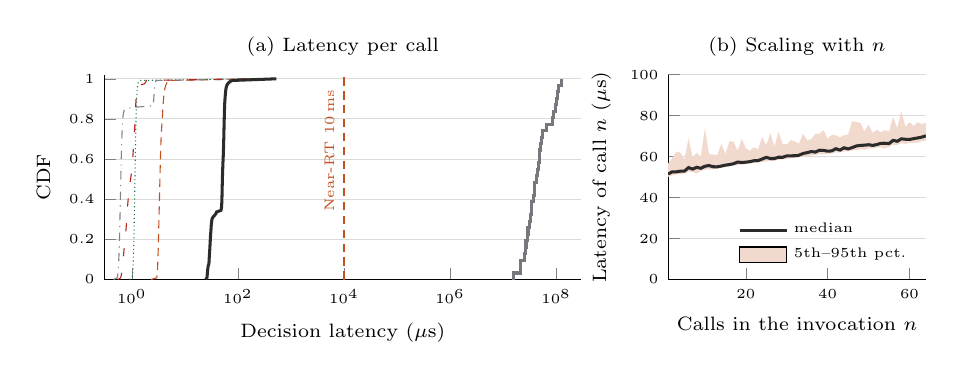
\begin{tikzpicture}
\begin{axis}[scale only axis, height=2.6cm, axis x line*=bottom, axis y line*=left, tick label style={font=\tiny}, label style={font=\scriptsize}, title style={font=\scriptsize, yshift=-1mm}, grid style={inkmuted!25}, ymajorgrids, width=0.5\columnwidth, name=cdf, xmode=log, xmin=0.3, xmax=3e+08, ymin=0, ymax=1.02,
  xtick={1,100,10000,1000000,100000000}, xlabel={Decision latency ($\mu$s)}, ylabel={CDF},
  title={(a) Latency per call},
  legend to name=legLatency, legend columns=3, legend cell align=left,
  legend style={font=\tiny, draw=none, /tikz/every even column/.append style={column sep=5pt}},
  xminorticks=false]
\addplot[detline, densely dashed, no marks] coordinates {(2.309,0.0000) (2.952,0.0084) (2.984,0.0168) (3.006,0.0252) (3.022,0.0336) (3.036,0.0420) (3.047,0.0504) (3.058,0.0588) (3.068,0.0672) (3.077,0.0756) (3.086,0.0840) (3.094,0.0924) (3.101,0.1008) (3.109,0.1092) (3.116,0.1177) (3.123,0.1261) (3.130,0.1345) (3.136,0.1429) (3.143,0.1513) (3.149,0.1597) (3.155,0.1681) (3.162,0.1765) (3.168,0.1849) (3.174,0.1933) (3.180,0.2017) (3.186,0.2101) (3.192,0.2185) (3.198,0.2269) (3.204,0.2353) (3.209,0.2437) (3.215,0.2521) (3.221,0.2605) (3.227,0.2689) (3.233,0.2773) (3.238,0.2857) (3.244,0.2941) (3.250,0.3025) (3.256,0.3109) (3.261,0.3193) (3.267,0.3277) (3.273,0.3361) (3.279,0.3445) (3.285,0.3529) (3.290,0.3613) (3.296,0.3698) (3.302,0.3782) (3.308,0.3866) (3.314,0.3950) (3.320,0.4034) (3.326,0.4118) (3.332,0.4202) (3.338,0.4286) (3.344,0.4370) (3.349,0.4454) (3.355,0.4538) (3.361,0.4622) (3.367,0.4706) (3.372,0.4790) (3.378,0.4874) (3.384,0.4958) (3.390,0.5042) (3.396,0.5126) (3.402,0.5210) (3.408,0.5294) (3.414,0.5378) (3.420,0.5462) (3.426,0.5546) (3.432,0.5630) (3.439,0.5714) (3.445,0.5798) (3.452,0.5882) (3.458,0.5966) (3.465,0.6050) (3.472,0.6134) (3.479,0.6219) (3.487,0.6303) (3.494,0.6387) (3.502,0.6471) (3.510,0.6555) (3.518,0.6639) (3.527,0.6723) (3.537,0.6807) (3.546,0.6891) (3.557,0.6975) (3.568,0.7059) (3.580,0.7143) (3.593,0.7227) (3.607,0.7311) (3.622,0.7395) (3.638,0.7479) (3.654,0.7563) (3.672,0.7647) (3.690,0.7731) (3.708,0.7815) (3.726,0.7899) (3.744,0.7983) (3.761,0.8067) (3.778,0.8151) (3.795,0.8235) (3.812,0.8319) (3.828,0.8403) (3.845,0.8487) (3.862,0.8571) (3.878,0.8655) (3.897,0.8740) (3.917,0.8824) (3.937,0.8908) (3.959,0.8992) (3.984,0.9076) (4.013,0.9160) (4.047,0.9244) (4.089,0.9328) (4.138,0.9412) (4.193,0.9496) (4.262,0.9580) (4.353,0.9664) (4.473,0.9748) (4.629,0.9832) (5.486,0.9916) (209.191,1.0000)};
\addlegendentry{$g_S$}
\addplot[okline, densely dotted, no marks] coordinates {(0.901,0.0000) (1.005,0.0084) (1.020,0.0168) (1.029,0.0252) (1.037,0.0336) (1.042,0.0420) (1.047,0.0504) (1.051,0.0588) (1.055,0.0672) (1.059,0.0756) (1.062,0.0840) (1.065,0.0924) (1.068,0.1008) (1.071,0.1092) (1.073,0.1177) (1.076,0.1261) (1.078,0.1345) (1.080,0.1429) (1.083,0.1513) (1.085,0.1597) (1.087,0.1681) (1.089,0.1765) (1.090,0.1849) (1.092,0.1933) (1.094,0.2017) (1.096,0.2101) (1.097,0.2185) (1.099,0.2269) (1.101,0.2353) (1.102,0.2437) (1.104,0.2521) (1.106,0.2605) (1.107,0.2689) (1.109,0.2773) (1.110,0.2857) (1.111,0.2941) (1.113,0.3025) (1.114,0.3109) (1.116,0.3193) (1.117,0.3277) (1.119,0.3361) (1.120,0.3445) (1.121,0.3529) (1.123,0.3613) (1.124,0.3697) (1.125,0.3782) (1.127,0.3866) (1.128,0.3950) (1.130,0.4034) (1.131,0.4118) (1.132,0.4202) (1.134,0.4286) (1.135,0.4370) (1.136,0.4454) (1.137,0.4538) (1.139,0.4622) (1.140,0.4706) (1.141,0.4790) (1.143,0.4874) (1.144,0.4958) (1.145,0.5042) (1.146,0.5126) (1.148,0.5210) (1.149,0.5294) (1.150,0.5378) (1.152,0.5462) (1.153,0.5546) (1.154,0.5630) (1.156,0.5714) (1.157,0.5798) (1.158,0.5882) (1.160,0.5966) (1.161,0.6050) (1.163,0.6134) (1.164,0.6219) (1.165,0.6303) (1.167,0.6387) (1.168,0.6471) (1.170,0.6555) (1.171,0.6639) (1.173,0.6723) (1.174,0.6807) (1.176,0.6891) (1.178,0.6975) (1.179,0.7059) (1.181,0.7143) (1.183,0.7227) (1.184,0.7311) (1.186,0.7395) (1.188,0.7479) (1.190,0.7563) (1.191,0.7647) (1.193,0.7731) (1.195,0.7815) (1.197,0.7899) (1.199,0.7983) (1.202,0.8067) (1.204,0.8151) (1.206,0.8235) (1.208,0.8319) (1.211,0.8403) (1.214,0.8487) (1.216,0.8571) (1.219,0.8655) (1.222,0.8739) (1.226,0.8824) (1.229,0.8908) (1.232,0.8992) (1.237,0.9076) (1.241,0.9160) (1.246,0.9244) (1.251,0.9328) (1.258,0.9412) (1.265,0.9496) (1.274,0.9580) (1.285,0.9664) (1.302,0.9748) (1.331,0.9832) (1.455,0.9916) (175.938,1.0000)};
\addlegendentry{$g_P$}
\addplot[llmfill!45!ink, dashdotted, no marks] coordinates {(0.453,0.0000) (0.528,0.0084) (0.538,0.0168) (0.544,0.0252) (0.548,0.0336) (0.552,0.0420) (0.555,0.0504) (0.558,0.0588) (0.560,0.0672) (0.563,0.0756) (0.565,0.0840) (0.567,0.0924) (0.568,0.1008) (0.570,0.1092) (0.572,0.1177) (0.573,0.1261) (0.575,0.1345) (0.576,0.1429) (0.577,0.1513) (0.579,0.1597) (0.580,0.1681) (0.581,0.1765) (0.583,0.1849) (0.584,0.1933) (0.585,0.2017) (0.586,0.2101) (0.587,0.2185) (0.588,0.2269) (0.589,0.2353) (0.590,0.2437) (0.591,0.2521) (0.593,0.2605) (0.594,0.2689) (0.595,0.2773) (0.596,0.2857) (0.597,0.2941) (0.597,0.3025) (0.598,0.3109) (0.599,0.3193) (0.600,0.3277) (0.601,0.3361) (0.602,0.3445) (0.603,0.3529) (0.604,0.3613) (0.605,0.3697) (0.606,0.3782) (0.607,0.3866) (0.608,0.3950) (0.609,0.4034) (0.610,0.4118) (0.611,0.4202) (0.611,0.4286) (0.612,0.4370) (0.613,0.4454) (0.614,0.4538) (0.615,0.4622) (0.616,0.4706) (0.617,0.4790) (0.618,0.4874) (0.619,0.4958) (0.620,0.5042) (0.621,0.5126) (0.622,0.5210) (0.623,0.5294) (0.624,0.5378) (0.625,0.5462) (0.626,0.5546) (0.627,0.5630) (0.628,0.5714) (0.629,0.5798) (0.630,0.5882) (0.631,0.5966) (0.632,0.6050) (0.634,0.6134) (0.635,0.6219) (0.636,0.6303) (0.637,0.6387) (0.638,0.6471) (0.640,0.6555) (0.641,0.6639) (0.643,0.6723) (0.644,0.6807) (0.645,0.6891) (0.647,0.6975) (0.648,0.7059) (0.650,0.7143) (0.652,0.7227) (0.654,0.7311) (0.656,0.7395) (0.658,0.7479) (0.660,0.7563) (0.662,0.7647) (0.665,0.7731) (0.668,0.7815) (0.671,0.7899) (0.675,0.7983) (0.679,0.8067) (0.684,0.8151) (0.690,0.8235) (0.698,0.8319) (0.712,0.8403) (0.746,0.8487) (1.011,0.8571) (2.498,0.8655) (2.534,0.8739) (2.558,0.8824) (2.575,0.8908) (2.591,0.8992) (2.605,0.9076) (2.619,0.9160) (2.632,0.9244) (2.645,0.9328) (2.658,0.9412) (2.673,0.9496) (2.689,0.9580) (2.709,0.9664) (2.733,0.9748) (2.767,0.9832) (2.844,0.9916) (271.508,1.0000)};
\addlegendentry{$g_L$}
\addplot[rejline, loosely dashed, no marks] coordinates {(0.548,0.0000) (0.615,0.0084) (0.627,0.0168) (0.636,0.0252) (0.644,0.0336) (0.650,0.0420) (0.656,0.0504) (0.662,0.0588) (0.667,0.0672) (0.672,0.0756) (0.677,0.0840) (0.681,0.0924) (0.686,0.1008) (0.690,0.1092) (0.695,0.1177) (0.700,0.1261) (0.705,0.1345) (0.709,0.1429) (0.714,0.1513) (0.719,0.1597) (0.724,0.1681) (0.730,0.1765) (0.735,0.1849) (0.741,0.1933) (0.747,0.2017) (0.752,0.2101) (0.758,0.2185) (0.763,0.2269) (0.769,0.2353) (0.774,0.2437) (0.778,0.2521) (0.783,0.2605) (0.787,0.2689) (0.791,0.2773) (0.795,0.2857) (0.799,0.2941) (0.803,0.3025) (0.807,0.3109) (0.811,0.3193) (0.815,0.3277) (0.819,0.3361) (0.822,0.3445) (0.827,0.3529) (0.831,0.3613) (0.835,0.3697) (0.840,0.3782) (0.845,0.3866) (0.850,0.3950) (0.855,0.4034) (0.861,0.4118) (0.867,0.4202) (0.875,0.4286) (0.882,0.4370) (0.890,0.4454) (0.897,0.4538) (0.906,0.4622) (0.915,0.4706) (0.924,0.4790) (0.933,0.4874) (0.943,0.4958) (0.953,0.5042) (0.962,0.5126) (0.972,0.5210) (0.981,0.5294) (0.990,0.5378) (0.998,0.5462) (1.005,0.5546) (1.012,0.5630) (1.018,0.5714) (1.024,0.5798) (1.030,0.5882) (1.036,0.5966) (1.041,0.6050) (1.046,0.6134) (1.052,0.6219) (1.057,0.6303) (1.063,0.6387) (1.068,0.6471) (1.074,0.6555) (1.079,0.6639) (1.085,0.6723) (1.090,0.6807) (1.096,0.6891) (1.101,0.6975) (1.106,0.7059) (1.111,0.7143) (1.116,0.7227) (1.120,0.7311) (1.125,0.7395) (1.129,0.7479) (1.134,0.7563) (1.137,0.7647) (1.141,0.7731) (1.145,0.7815) (1.149,0.7899) (1.153,0.7983) (1.156,0.8067) (1.160,0.8151) (1.164,0.8235) (1.167,0.8319) (1.171,0.8403) (1.175,0.8487) (1.179,0.8571) (1.183,0.8655) (1.187,0.8739) (1.191,0.8824) (1.196,0.8908) (1.201,0.8992) (1.206,0.9076) (1.212,0.9160) (1.219,0.9244) (1.227,0.9328) (1.236,0.9412) (1.250,0.9496) (1.270,0.9580) (1.319,0.9664) (1.718,0.9748) (1.831,0.9832) (1.894,0.9916) (172.589,1.0000)};
\addlegendentry{$g_R$}
\addplot[ink, line width=1.1pt, no marks] coordinates {(24.907,0.0000) (26.084,0.0084) (26.288,0.0168) (26.461,0.0252) (26.640,0.0336) (26.820,0.0420) (27.002,0.0504) (27.209,0.0588) (27.528,0.0672) (28.214,0.0756) (28.483,0.0840) (28.620,0.0924) (28.727,0.1008) (28.829,0.1092) (28.933,0.1177) (29.060,0.1261) (29.203,0.1345) (29.363,0.1429) (29.506,0.1513) (29.633,0.1597) (29.752,0.1681) (29.866,0.1765) (29.983,0.1849) (30.095,0.1933) (30.211,0.2017) (30.330,0.2101) (30.467,0.2185) (30.629,0.2269) (30.815,0.2353) (30.986,0.2437) (31.124,0.2521) (31.260,0.2605) (31.399,0.2689) (31.586,0.2773) (31.860,0.2857) (32.199,0.2941) (32.647,0.3025) (33.813,0.3109) (36.213,0.3193) (38.446,0.3277) (39.371,0.3361) (47.794,0.3445) (48.773,0.3529) (49.132,0.3613) (49.400,0.3698) (49.596,0.3782) (49.749,0.3866) (49.873,0.3950) (49.976,0.4034) (50.075,0.4118) (50.166,0.4202) (50.251,0.4286) (50.332,0.4370) (50.415,0.4454) (50.500,0.4538) (50.582,0.4622) (50.667,0.4706) (50.757,0.4790) (50.851,0.4874) (50.949,0.4958) (51.054,0.5042) (51.160,0.5126) (51.272,0.5210) (51.387,0.5294) (51.505,0.5378) (51.629,0.5462) (51.760,0.5546) (51.895,0.5630) (52.039,0.5714) (52.195,0.5798) (52.369,0.5882) (52.549,0.5966) (52.724,0.6050) (52.885,0.6134) (53.037,0.6219) (53.170,0.6303) (53.296,0.6387) (53.425,0.6471) (53.541,0.6555) (53.656,0.6639) (53.769,0.6723) (53.879,0.6807) (53.982,0.6891) (54.087,0.6975) (54.182,0.7059) (54.274,0.7143) (54.367,0.7227) (54.459,0.7311) (54.547,0.7395) (54.632,0.7479) (54.721,0.7563) (54.811,0.7647) (54.904,0.7731) (55.002,0.7815) (55.101,0.7899) (55.202,0.7983) (55.306,0.8067) (55.411,0.8151) (55.520,0.8235) (55.627,0.8319) (55.740,0.8403) (55.864,0.8487) (56.000,0.8571) (56.148,0.8655) (56.319,0.8740) (56.532,0.8824) (56.794,0.8908) (57.098,0.8992) (57.423,0.9076) (57.758,0.9160) (58.093,0.9244) (58.456,0.9328) (58.886,0.9412) (59.501,0.9496) (60.405,0.9580) (61.658,0.9664) (64.063,0.9748) (68.551,0.9832) (77.914,0.9916) (532.472,1.0000)};
\addlegendentry{Gate (all)}
\addplot[llmfill!40!ink, line width=1.1pt, const plot, no marks] coordinates {(15881381.0,0) (15881381.0,0.0323) (21429220.0,0.0645) (21566616.0,0.0968) (24832297.0,0.1290) (26510364.0,0.1613) (27018580.0,0.1935) (28670792.0,0.2258) (29464513.0,0.2581) (31923105.0,0.2903) (32691479.0,0.3226) (34414824.0,0.3548) (34476695.0,0.3871) (38018503.0,0.4194) (39061862.0,0.4516) (39392443.0,0.4839) (42021841.0,0.5161) (44069773.0,0.5484) (46285974.0,0.5806) (47841143.0,0.6129) (48046524.0,0.6452) (51385903.0,0.6774) (53124769.0,0.7097) (55720809.0,0.7419) (65780322.0,0.7742) (85404349.0,0.8065) (90374965.0,0.8387) (98168713.0,0.8710) (100253868.0,0.9032) (104415764.0,0.9355) (111729592.0,0.9677) (124487490.0,1.0000)};
\addlegendentry{Gate + $g_V$ (live)}
\draw[detline, densely dashed, line width=0.5pt] (axis cs:1e4,0) -- (axis cs:1e4,1.02);
\node[font=\tiny, text=detline, rotate=90, anchor=south east, xshift=-0.5pt] at (axis cs:1e4,1.0) {Near-RT 10\,ms};
\end{axis}
\begin{axis}[scale only axis, height=2.6cm, axis x line*=bottom, axis y line*=left, tick label style={font=\tiny}, label style={font=\scriptsize}, title style={font=\scriptsize, yshift=-1mm}, grid style={inkmuted!25}, ymajorgrids, width=0.27\columnwidth, at={(cdf.east)}, anchor=west, xshift=11mm, xmin=1, xmax=64, ymin=0, ymax=100,
  xlabel={Calls in the invocation $n$}, ylabel={Latency of call $n$ ($\mu$s)},
  title={(b) Scaling with $n$},
  legend style={font=\tiny, draw=none, fill=none, at={(0.98,0.03)}, anchor=south east}, legend cell align=left]
\addplot[fill=detline!22, draw=none, forget plot] coordinates {(1,50.12) (2,50.90) (3,51.34) (4,51.62) (5,51.68) (6,52.70) (7,52.55) (8,51.70) (9,53.18) (10,53.56) (11,53.83) (12,53.85) (13,54.09) (14,54.50) (15,54.95) (16,55.20) (17,55.71) (18,55.78) (19,56.07) (20,56.40) (21,56.63) (22,56.92) (23,57.01) (24,57.41) (25,57.62) (26,57.96) (27,57.97) (28,58.49) (29,58.62) (30,58.89) (31,59.26) (32,59.41) (33,59.63) (34,60.14) (35,60.21) (36,60.62) (37,60.76) (38,61.22) (39,61.06) (40,61.44) (41,61.56) (42,62.13) (43,62.00) (44,62.63) (45,62.57) (46,63.01) (47,63.26) (48,63.58) (49,63.36) (50,64.07) (51,63.92) (52,64.48) (53,64.54) (54,63.95) (55,64.85) (56,65.71) (57,65.74) (58,66.60) (59,66.21) (60,66.76) (61,66.78) (62,66.90) (63,67.57) (64,67.73) (64,76.42) (63,76.00) (62,76.83) (61,74.94) (60,76.93) (59,74.60) (58,82.30) (57,73.96) (56,79.43) (55,72.28) (54,72.93) (53,72.04) (52,73.16) (51,71.62) (50,75.67) (49,72.30) (48,76.58) (47,76.84) (46,77.41) (45,70.77) (44,70.57) (43,69.34) (42,70.54) (41,70.64) (40,68.81) (39,72.88) (38,71.27) (37,71.24) (36,68.62) (35,67.98) (34,71.31) (33,66.40) (32,67.43) (31,68.07) (30,66.04) (29,66.29) (28,72.14) (27,64.99) (26,71.50) (25,65.53) (24,69.55) (23,63.65) (22,64.61) (21,62.86) (20,64.05) (19,68.76) (18,63.02) (17,67.26) (16,67.59) (15,61.32) (14,66.25) (13,60.77) (12,61.05) (11,61.25) (10,73.97) (9,60.04) (8,62.00) (7,59.51) (6,68.93) (5,58.62) (4,62.02) (3,62.51) (2,59.30) (1,56.66)} -- cycle;
\addplot[ink, line width=1.1pt, no marks] coordinates {(1,51.53) (2,52.60) (3,52.58) (4,52.91) (5,52.94) (6,54.66) (7,53.93) (8,54.80) (9,54.32) (10,55.32) (11,55.67) (12,55.08) (13,55.04) (14,55.40) (15,55.87) (16,56.13) (17,56.56) (18,57.37) (19,57.17) (20,57.31) (21,57.57) (22,58.02) (23,58.09) (24,58.86) (25,59.65) (26,59.09) (27,59.11) (28,59.73) (29,59.69) (30,60.39) (31,60.42) (32,60.46) (33,60.70) (34,61.58) (35,61.98) (36,62.50) (37,62.25) (38,63.14) (39,63.05) (40,62.68) (41,62.81) (42,63.89) (43,63.21) (44,64.33) (45,63.79) (46,64.44) (47,65.22) (48,65.50) (49,65.62) (50,65.83) (51,65.51) (52,65.89) (53,66.52) (54,66.56) (55,66.40) (56,67.96) (57,67.51) (58,68.71) (59,68.50) (60,68.39) (61,68.80) (62,69.15) (63,69.54) (64,70.20)};
\addlegendentry{median}
\addlegendimage{area legend, fill=detline!22, draw=none}
\addlegendentry{5th--95th pct.}
\end{axis}
\end{tikzpicture}\\[0.5mm]
\ref{legLatency}

\caption{Latency of the Trust \& Governance gate. (a) CDF per deterministic stage and for the whole deterministic gate (guards, proposal, $g_S$--$g_R$, audit; 52 live calls replayed through the unmodified middleware, $g_V$ disabled), and of the whole gate with $g_V$ in the live runs (31 calls, LangSmith traces). (b) Latency of a call as a function of its position $n$ in its invocation (deterministic gate).}
\label{fig:latency}
\end{figure}

\noindent \textbf{Gate latency.} Filtering these calls must not slow down control. To measure the deterministic gate precisely, we replay the 52 live calls through it with $g_V$ disabled, 5{,}000 times each on an Intel Core i7-10870H; the replay reproduces all 52 stored decisions. The deterministic gate decides in 51\,$\mu$s at the median and 74\,$\mu$s at the 99th percentile, each stage taking under 4\,$\mu$s (Fig.~\ref{fig:latency}a), i.e., over two orders of magnitude below the 10\,ms Near-RT budget. It grows only from 52 to 70\,$\mu$s when a call is the 64th of its invocation (Fig.~\ref{fig:latency}b). With $g_V$, the traces of the live runs show 42\,s at the median for the 31 calls that reached the review, almost entirely the model call itself. The safety checks are thus nearly free, the LLM review dominates the latency, and the 21 calls rejected by code never wait for it.

\noindent \textbf{Cost.} Finally, records without violation make no model call. For a violated record, the optimized configuration reduced the cost from 117\,k to 86\,k tokens ($-26$\%) and the agent time from 501 to 273\,s; most of the remaining tokens come from the Near-RT tool loop and the model's reasoning.

% =====================================================================
%\section{Discussion and Limitations}\label{sec:disc}
%\noindent \textbf{Design implications.} (i) Facts must stay with code: the LLM routed every violation correctly yet called most violated records ``normal''. (ii) A live LLM keeps the gate busy, 56\% of its calls being rejected, and two guards it exposed, no resubmission after a $g_V$ rejection and consistency with the controls in force, are deterministic and cheap. (iii) Authorization is \emph{slice-scoped}: a call may only act on the slice whose violation it answers. (iv) Numbers quoted in rationales and the bottleneck behind a tool choice can also be checked by code instead of $g_V$, which approved off-diagnosis calls. (v) A call budget should end the invocation, not only reject calls, and the reasoning effort of structured roles (Monitoring, $g_V$) should be limited: these are the two largest costs. (vi) LLM inference does not meet Near-RT timescales, so ``Near-RT'' is a role here.

%\noindent \textbf{Limitations.} The live evidence is small: one model, 11 violated records of one cell, slice and configuration, on a free endpoint whose rate limits stopped runs. It is open-loop: the tool calls change nothing, so we measure decisions and the gate, not their effect on the SLA. ColO-RAN uses static UEs and a fixed traffic mix, queueing delay is estimated from buffer occupancy, and the SLA budgets are our choice. The scores are rule-based heuristics with stated thresholds and await expert ratings. The evaluation scripts are released.

%\noindent \textbf{Design implications.} (i) \emph{Keeping facts in code pays off}: the LLM routed every violation correctly, and code corrected its situation labels before any action (P1). (ii) \emph{The gate is essential with a live LLM}: it filtered 56\% of the calls, and the guards added from live runs (no resubmission after a $g_V$ rejection, consistency with the controls in force) cost only microseconds. (iii) \emph{More checks can move into code}: quoted numbers and the bottleneck behind a tool choice are verifiable deterministically, reducing the reliance on $g_V$. (iv) \emph{Cost and timing are configurable}: a call budget that ends the invocation and a bounded reasoning effort cut the main costs, and while the gate meets Near-RT budgets, LLM inference sets the agents' pace, so ``Near-RT'' denotes their role.


%\noindent \textbf{Limitations and future work.} This study focuses on validating the architecture and the gate end to end with a live LLM, on 11 violated records of one cell and slice configuration with one model; extending it to more cells, slices and models is ongoing. The evaluation is open-loop, so it measures the agents' decisions and the gate rather than their effect on the SLA; closing the loop on an O-RAN testbed through E2/A1 is our next step. ColO-RAN uses static UEs and a fixed traffic mix, and the SLA budgets follow its traffic classes. The rule-based scores use stated thresholds and will be complemented by expert ratings; all evaluation scripts are released.

% =====================================================================
\section{Conclusion}
We presented \fw{}, a trust-gated multi-agent LLM architecture for O-RAN slice assurance in which deterministic grounding and a fail-closed gate bracket LLM orchestration and action proposal, with an LLM review as the last stage. Running the complete system with a live LLM on records from a real RAN stack, the gate held every invariant while rejecting 56\% of the calls, code overrode the orchestrator's situation label in 8 of 11 violated records, and compact prompts with a call budget cut the cost per record by 26\%. Future work will measure run-to-run stability and compare models on the same records, move the diagnosis and number checks into code, and close the loop on an O-RAN testbed through E2/A1.

\bibliographystyle{IEEEtran}
\bibliography{references}

\end{document}
